%!TEX root = main.tex

\section{Implementing bcrypt on FPGAs}
\label{sec:implementation}

In this section, we describe our FPGA implementation of a multi-core bcrypt
cracker, capable of both on-chip password generation and offline dictionary
attacks. We start with the general design decisions, the results of an early
version of our design and discuss the choices we made to improve the overall
design.

An efficient implementation should result in a balanced usage of the available
dedicated hardware and fabric resources and maximize the number of parallel
instances on the device. In the case of bcrypt, using one dual-port BRAM
resource to store two SBoxes saves LUT resources, results in high clock
frequencies and relaxes the routing without creating wait-states. To increase
the utilization of the memory, we focused on shared memory access without adding
clock cycles to the main computation. In the final design, one bcrypt core
occupies three BRAM blocks with two additional global memory resources for the
initialization values. This leads to an upper bound of 46 cores per zedboard
(ignoring any extra BRAM usage of the interface).

Considering a brute-force attack to benchmark the capabilities of the FPGA, the
interface can be minimalistic. We use a bussystem with minimal bandwidth
capacity, resulting in a small on-chip area footprint. For this scenario, we
chose the following setup: During start-up, the host transfers a 128-bit target
salt and a 192-bit target hash to the FPGA. These values are kept in two
registers to allow access during whole computation time. After filling the
registers, all bcrypt cores start to work in parallel. The password candidates
are generated on-chip. When the attack completes, a successful candidate is
transferred back to the host.

Our earlier design was built out of fully independent bcrypt cores. Each core
contained its own password register as well as the memory for the initialization
values. This effectively removed all cross-dependencies and resulted in very
short routing delays and thus very high clock frequencies. Due to Blowfish's
simple Feistel structure, only a small amount of combinatoric logic was needed:
Since the main work is done via BRAM lookups. Nevertheless, storing the password
in fabric consumes far too much area and resulted in an unbalanced
implementation. However, the timing results indicated that more than 100 MHz
should be possible.

\begin{figure}[tp] \centering
	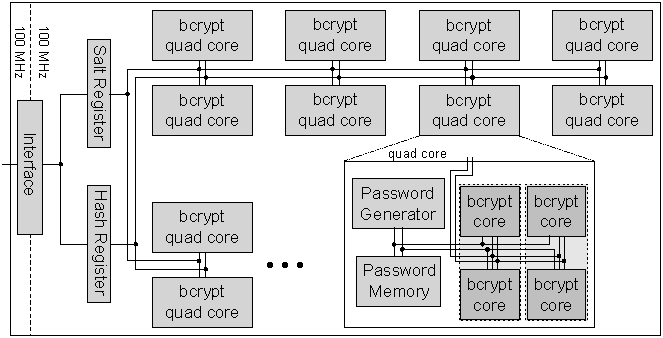
\includegraphics[width=0.475\textwidth]{figures/bcrypt_design_overview.pdf}
	\caption{Schematic Top-Level view of FPGA implementation. The design
	uses multiple clock-domains: a (slow) interface clock and a fast bcrypt
	clock. Each quad-core accesses the salt- and hash registers and consists of 
	a dedicated password memory, four bcrypt cores and a password generator.}
	\label{fig:bcrypt_design_overview}
\end{figure}

In order to reduce the area footprint, we tried to share resources and
analyzed the algorithm for registers that are not constantly accessed by all
cores. We first removed the initialization memory and used the free register
resources to implement a pipeline and buffer the signals such that the critical
path was unaffected by the change. Due to the required memory access and the
dual port properties, we also combined four bcrypt cores with one password
generator and password memory. These \emph{quad-cores} can schedule password
accesses with negligible overhead.

\begin{figure*}[tp] \centering
	\begin{minipage}[b]{0.45\textwidth} \centering
		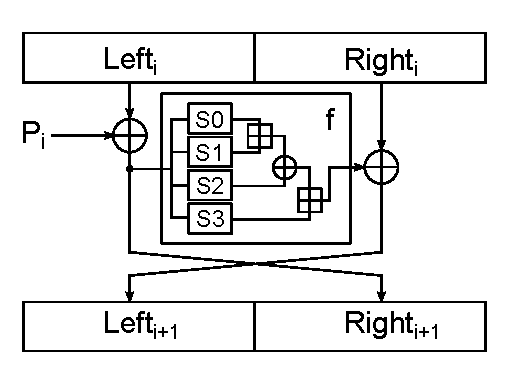
\includegraphics[height=3.5cm]{figures/blowfish_feistel.pdf}
		\caption{The normal Feistel-structure of one standard Blowfish round.
		         Note that the final XOR operation may be moved along the datapath.
				 By delaying it to the next round, we can resolve data
				 dependencies and compute one Blowfish round in one clock
				 cycle more efficiently.}
		\label{fig:blowfish-feistel}
	\end{minipage}%
	\hspace{0.5cm}
	\begin{minipage}[b]{0.45\textwidth} \centering
		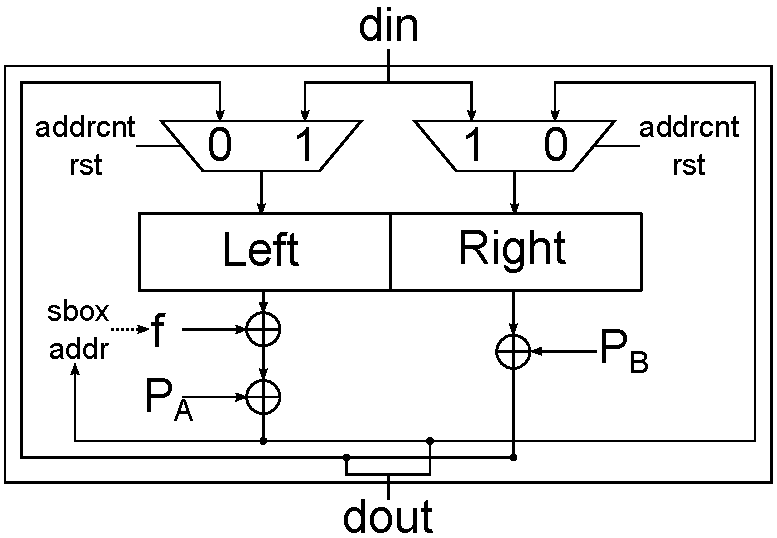
\includegraphics[height=3.5cm]{figures/blowfish_core.pdf}
		\caption{Blockdiagram of Blowfish core. The computation of the delayed 
                 f-function is integrated into the left half and the result of
				 the modified data-path forms the memory address for the next f-function.}
		\label{fig:blowfish-core}
	\end{minipage}
\end{figure*}

These changes reduced the area consumption by roughly 20\% at the cost of one
additional BRAM resource per quad-core. Figure~\ref{fig:bcrypt_design_overview}
shows the resulting design using multiple parallel and independent quad-cores.
Every bcrypt core starts its operation with the initialization of the 256 SBox
entries. Within this timeslot, the password generator produces four new
passwords and writes them into the password memory. By using the dual-port
structure of the memory, two bcrypt cores access their passwords in parallel.
While these first two cores uses the BRAM, the second pair of cores is stalled.
This leads to a delay of 19 clock cycles between both pairs.

The bcrypt core spents most of the time within Blowfish encryptions, as these
are used during the \texttt{ExpandKey} (521 times) and \texttt{EncryptECB} (3
times) steps. Thus, optimizing the Blowfish core heavily improves the overall
performance. A na\"ive implementation needs two clock cycles per Blowfish round:
one to calculate the input of the f-function -- and thus the addresses to the
SBox entries -- and one to compute the XOR operation on the f-function output
and the subkey.

Figure~\ref{fig:blowfish-feistel} shows the standard Blowfish Feistel round. We
moved the XORs along the datapath, changing the round boundaries. This delay
allows us to prefetch the subkeys from the memory and resolve data-access
dependencies to reduce the cycle count to one per round.

The resulting Blowfish core is depicted in Figure~\ref{fig:blowfish-core}. All
of the three XOR operations -- the f-function's output and the subkeys
$\text{P}_\text{A}$ and $\text{P}_\text{B}$ -- are computed in every round,
removing all multiplexers from the design. As this would change the Blowfish
algorithm, we use the reset of the BRAM output registers to suppress any invalid
XOR operations during the computation. This design leads to a very minimalistic
control logic and a very small Blowfish design in terms of area. Concerning the
critical path, the maximum delay comes from the path from the SBox through the
evaluation of the f-function.
%\footnote{To address this problem, we designed a
%pipelined, interleaved Blowfish module, which all four cores of the quad-core
%share. These results are still pending and will be included later, if the
%paper is accepted and the addition is allowed.}

We have roughly a fourth of the available slices left when we reach the limit of
available memory blocks. These resources can be utilized for the password
generation. In its simplest form, this is very efficient on-chip, as it only
requires a small amount of logical resources.
%Figure~\ref{fig:password_generation} provides a schematic overview.
For each  password byte, one counter and register store the current states. The
initialization value differs for every core and determines the search space. The
logic always generates two subsequent passwords and enumerates over all possible
combinations for a given character set and maximum password length. When the
state has been updated correctly, it is mapped into ASCII representation and
written into the password memory. The generation process finishes during the 256
initialization clock cycles, leaving enough time to buffer the signals and
ensure a low amount of levels-of-logic.

%\begin{figure}[tp] \centering
%	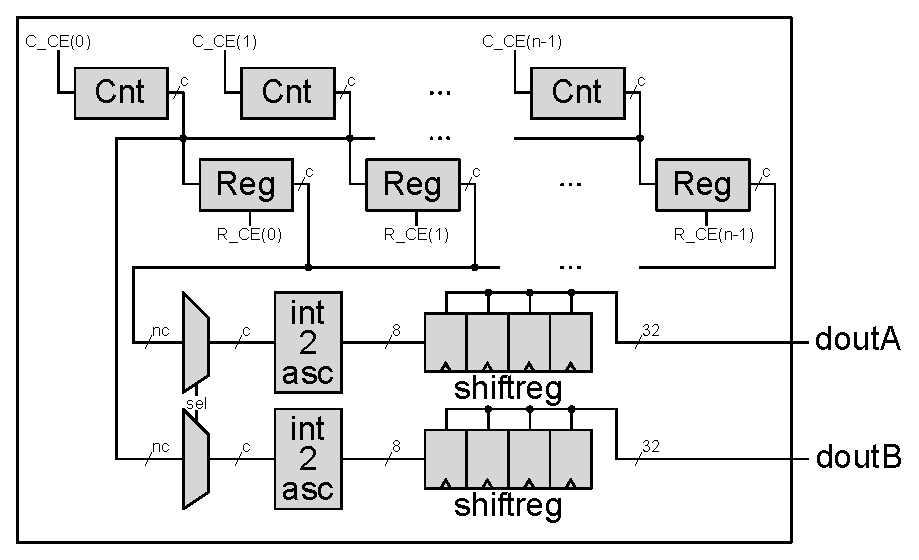
\includegraphics[width=0.475\textwidth]{figures/password_gen.pdf}
%	\caption{Schematic view of the password generation. The counter and registers in
%	the upper half store the actual state of the generator. The mapping to ASCII
%	characters is done by multiplexer. It uses a cyclic output for bcrypt and
%	generates two passwords in parallel.}
%	\label{fig:password_generation}
%\end{figure}

Please note that with this design, even a slow and simple interface capable of
sending 320 bits and a start flag can use the system for brute-force attacks.
A more complex interface -- capable of fast data-transfer or even direct memory
access of the BRAM cores -- easily enables dictionary attacks, as new
passwords are transferred directly into the password memory during the long
bcrypt computation. The on-chip password generation may be removed or modified
to work in a hybrid mode.
